\section{Research Implementation} 
In this section we describe the architecture of of CARLA in detail and the present our fault injection methodology. 

\subsection{CARLA} \label{ri-carla}
CARLA is an open source simulator built on Unreal Engine 4. CARLA provides simulation of realistic physics, NPC logic and dynamic world. CARLA simulates actions of an autonomous vehicle (AV) and the environment that this AV experiences, with ability to control the actions of the AV by an external driving agent,  that decides actions to be taken by AV, based on the data that it retrieves from simulation engine. Figure~\ref{fig:carla_arch} shows the high level architecture of CARLA. CARLA operates in a server-client model, with functionality between these divided in following manner.

\subsubsection{Client} It runs the simulation and renders the environment that the AV experiences.

\subsubsection{Server} It controls the parameters of the simulation and also controls the actions of the AV based on predefined algorithms. 

\begin{figure}  [h]
	\vspace{-0.5em}
	\centering
	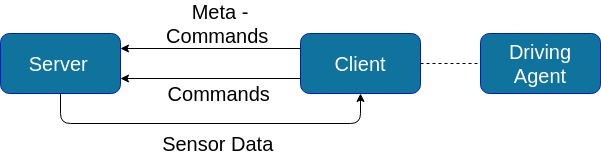
\includegraphics[scale=0.4]{CARLA_block}
	\vspace{-0.5em}
	\caption{High level architecture of CARLA}
	\label{fig:carla_arch}
	\vspace{-1.5em}
\end{figure}

\bigskip

Due to this client-server architecture CARLA provides flexibility to swap multiple driving algorithms (called driving agents in CARLA terminology) and driving environments easily. The server provides the ability to render a range of environments by changing the weather, number of vehicles and pedestrians etc in the simulation environment. The server also provides the output of various sensors attached to AV to the driving agent. The client connects to the server using sockets and provides two type of inputs, commands and meta-commands, to the server. Commands control the behavior of the vehicles i.e braking, steering, accelerating etc. and are provided by the driving agent which is integrated with client side in CARLA using python APIs. Meta-commands are used to control the behavior of simulation.

Although CARLA provides ability to simulate complex environments, Dosovitskiy et al.~\cite{Dosovitskiy17} have shown that for a range of driving agents, only simple paths with no dynamic actors present produce successful results for more than 90 percent trials. Following this information we primarily select the following environmental conditions for our experiments. 

The ideal destination of vehicle is on the same line as the starting points with a distance of 200m and no dynamic objects are present in the simulation.

\subsection{Driving Agent}
As mentioned in the previous section the behavior of the vehicle in te simulation is controlled by the driving agent. As we want to study the resilience of CARLA, we have chosen an already developed driving agent, which uses conditional imitation learning to train a deep neural network~\cite{Codevilla2018}, which after offline training, is used for inferencing for taking decision during simulation. We take an already trained model and use that in our Fault injection phase. Dosovitskiy et al.~\cite{Dosovitskiy17} have shown that success rate of the trained driving agent for the chosen environmental conditions is greater than 95\%.

\subsection{Fault Injection method} \label{method}
As mentioned in~\ref{ri-carla} CARLA provides a client server architecture. We exploit this boundary between client and server for our fault injection experiments. 

\begin{figure}  [h]
	\vspace{-0.5em}
	\centering
	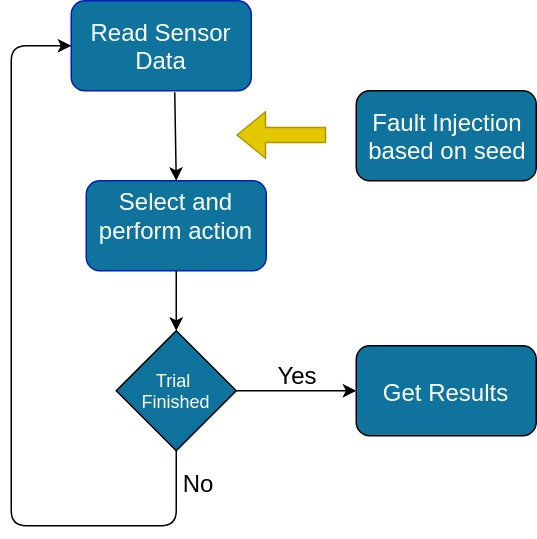
\includegraphics[scale=0.3]{FI_method}
	\vspace{-0.5em}
	\caption{Fault injection method used in experiments}
	\label{fig:FI_method}
	\vspace{-1.5em}
\end{figure}

Figure~\ref{fig:FI_method} provides an overview of method of fault injection used in one trial. The CARLA platform provides an ability to run multiple trails of the same experiments (same environment and goals). Each trial involves multiple steps. In each step data is read from the sensors, this data is provided to the controller which based on some predefined algorithm and current sensor readings, gives command to the AV, after the command its checked if the objective of the trial is achieved or the timeout has happened. If any of these condition exists we end the current trial and the using the measurements from the server, the metrics defined in~\ref{fi_m} are calculated for this trial and after that we move on to the next trial. 

The sensor readings are provided in form of dictionary to driving agent from the client, which can be easily accessed in the code. We insert a code block in between reading data from server and sending it to driving agent. This code block changes the reading of the sensor under study based on the fault that we are testing. This code block injects fault in only one step during each trial, as we intend to study the effect of individual faults. 

The fault space for even one sensor using approach mentioned above is quite big, which may lead to state space explosion. We intend to use this approach as a stepping stone towards finding a systematic approach for FI.  

\subsection{Constraints}
 